\cotefile{156-7}
\scanpage{10}\mspage{9}
Forme affaiblie de la Propriété 1

\deleted{\uline{At CD 1'} Soient $x,y,x$}

\noindent\begin{tabular}{|p{.93\linewidth}}
\uline{Propriété} $1^{\unsure{\prime}}_{0}$\quad $F,\unsure{G|C},F',G'$ avec $F\mathrel{>\mkern-12mu<}G$, $F'\ll F$, $G'\ll G$. Posons $L=F\cap G$, \deleted{et supposons $F'_L\parallel G'_L$} Alors
\[
F'\parallel G'\Longleftrightarrow F'_L\parallel G'_L
\]
\end{tabular}

L'implication $\Rightarrow$ tjrs valable. \inserted{la validité de} L'implication en sens \unsure{inverse} \unsure{équivaut} \unsure{:|à}

% slanted
\margin{\uline{Critère de disjonction pour les \unsure{raffinements} de sous-figures}}
\noindent\begin{tabular}{||p{.92\linewidth}}
\uline{At CD} $1^{\prime}_{0}$\quad Soient $x,y,x',y'\in\unsure{M|\mathcal{M}}$, $x\mathrel{>\mkern-12mu<}y$, $x'\ll x$, $y'\ll y$. Posons $L=x\cap y$ et supposons que $x'_L\parallel y'_L$ (i.e. $\forall\,x'',y''\in M$, $x''\leq x'$, $y''\leq y'$, $x'''\ll L$, $y''\ll L$, on ait $x''\parallel y''$) Alors $x'\parallel y'$ \unsure{(NB} \unsure{réciproque|récipr. que|récipr. qui} tjrs vraie !)\unsure{*}
\inserted{$=$ \unsure{sans} At CD 1')}
\end{tabular}

\uline{Cor. 1}\quad Validité de Propriété $1'$

\uline{Cor. 2}\quad Si $F,G,\deleted{\unsure{\in}}F'\in\mathcal{F}$, avec $F\mathrel{>\mkern-12mu<}G$, $F'\ll F$, \unsure{supposant} $F'_L=\unsure{\phi|\varnothing}_{\mathcal{F}}$ (où $L=F\cap G$), alors $F'$ est disjoint de tout \unsure{raffinement} $G'$ de $G$

\uline{Cor. 3}\quad \unsure{Soient|Soit} $F\parallel G$, alors $F'\ll F$, $G'\ll G\Rightarrow F'\parallel G'$.

% slanted
\margin{\uline{Corollaire} 4\\ Soient
\diagram{\begin{tikzcd}[ampersand replacement=\&,row sep=0pt,column sep=.1em]
F' \& \ll \& F \\
\& \& {\unsure{\tikz[x=.5em,y=.5em,baseline=-.3ex]{\draw (0,1)--(.4,0)--(.9,1) (.67,-.22)--(1.15,.78);}}} \\
\& \& {\deleted{\unsure{G|F}}L}
\end{tikzcd}}.
Pour que $F'_L=\phi_{\mathcal{F}}$, il f. et \unsure{s.|S.} que $F'\parallel L$. (le il suffit vrai \unsure{sans} axiomes suppl., c'est le ``il faut'' ou $F'_L=\phi_{\mathcal{F}}\Rightarrow F'\parallel L$ qui demande \unsure{``l'axiome''}\unsure{...})}

\unsure{J'ai} tendance à \unsure{regarder} At CD comme ``axiomes \unsure{obligatoires}'' pour les ateliers.

\deleted{\uline{At CD} 2 (Axiome des ateliers spacieux)}

\noindent\begin{tabular}{|p{.93\linewidth}}
\uline{Propriété} 2 (des ``ateliers spacieux''). Soient $F,G\in\mathcal{F}$, \deleted{\illegible{1}} on ne suppose pas $F\mathrel{>\mkern-12mu<}G$, mais soit $L=F\cap G=\displaystyle\mathop{\mathrm{Sup}}_{\unsure{Z|z}\,\in\,\widetilde F\cap\widetilde G} Z$. \deleted{$\unsure{A}$} Supposons que pour tout $F'\ll F$ tel que $F'_L=\phi_{\mathcal{F}}$ (i.e. $\overbrace{F'\parallel L}^{\text{\inserted{par At CD 1',}}}$) et $G'\ll G$ tel que $G'_L=\phi_{\mathcal{F}}$ (\unsure{i.e.} $G'\parallel L$) on ait $F'\parallel G'$. Alors $F\mathrel{>\mkern-12mu<}G$.
\end{tabular}
\scanpage{11}\mspage{10}
Pour ceci, il \inserted{\unsure{faut et|f. et}} suffit qu'on ait l'axiome suivant

% slanted
\margin{Critère de compatibilité absolue des ateliers spacieux}
\uline{At CD 2}\quad Soient $x,y\deleted{\unsure{,}}\in\unsure{M|\mathcal{M}}$, \deleted{\unsure{soit}} on ne suppose pas $x\deleted{\mathrel{>\mkern-12mu<}}y$ compatibles mais on introduit $K=x\cap y=\displaystyle\mathop{\mathrm{Sup}}_{\unsure{z|Z}\,\in\,\widetilde x\cap\widetilde y}z$. On suppose que pour tout $x',y'\in M$ avec $x'\ll x$, $x'_L=\unsure{\phi|\varnothing}_{\mathcal{F}}$ et $y'\ll y$, $y'_L=\phi_{\mathcal{F}}$, on ait $x'\deleted{\mathrel{>\mkern-12mu<}}\parallel y'$. \deleted{\inserted{\illegible{2}}} Alors $x\mathrel{>\mkern-12mu<}y$.

Cet axiome n'est pas satisfait \inserted{le plus \unsure{souvent}} pour les \uline{ateliers} dits ``\uline{\unsure{polyédraux}}'', i.e. satisfaisant \unsure{à :|:} \deleted{\unsure{pour} tout} \inserted{deux} multistrates, \deleted{\unsure{doivent être des} \illegible{1}} \inserted{compatibles, minorés} \deleted{\unsure{disjointes|disjoints}} ont pour intersection une \unsure{multistrate}
i.e. si $x,y$ \deleted{$\unsure{\in M}$} dans $M$ \deleted{et \illegible{1} $x,y$ \unsure{majorés}} \inserted{avec $x\mathrel{>\mkern-12mu<}y$}, \deleted{\unsure{et}} \inserted{et} minorés dans $M$ \inserted{(pas néc. \unsure{majorés})}, alors \deleted{inf dans $M$} $x,y$ ont un inf dans $M$ i.e. $x\underset{\mathcal{F}}{\cap}y\in M$. Pour ceux-ci, \unsure{posera}

% slanted
\margin{Critère de compatibilité absolue \unsure{des|aux|dans} ateliers \unsure{polyédraux}}
\uline{At CD} $2'$ \quad Soient $x,y\in M$, $K=x\cap y=\displaystyle\mathop{\mathrm{Sup}}_{z\,\in\,\widetilde x\cap\widetilde y}z$. On suppose que $\forall\,x',y'\in M$, $x'\ll x$, $x'_L=\phi_{\mathcal{F}}$, $y'\ll y$, $y'_L=\phi_{\mathcal{F}}$, on ait $x'\parallel y'$. \deleted{Alors $x\mathrel{>\mkern-12mu<}y$.} Supposons de plus $K\in M$ i.e. c'est un $\mathrm{inf}^{\unsure{\leq}}$ de $x,y$ dans $\deleted{\unsure{Z}}M$. Alors $x\mathrel{>\mkern-12mu<}y$.

\deleted{\uline{NB} Chacune de ces deux conditions implique \uline{At CD} $1_0$.}

\noindent\begin{tabular}{||p{.92\linewidth}}
\uline{N.B.} \unsure{Tous} les ateliers que j'ai \unsure{vus} comme \unsure{motivants} satisfont At CD $1_0$, et l'un des deux axiomes At CD 2 ou At. CD $2'$.
\end{tabular}

% slanted
\margin{Attention La relation $\parallel$ \uline{dans $M$} ne résulte pas (comme dans $\unsure{\overline{F}|\mathcal{F}}$) de la seule donnée de $\leq$ -- ici il faut la voir (\unsure{en|ou} l'absence \unsure{en général|en la définition} de $\unsure{\widehat F|\overline F}$ \unsure{ou|en} $\unsure{b_{\overline{0}}|b_0}$) comme une \unsure{donnée} \uline{primitive}.}
L'intérêt de At CD, c'est de ramener la relation $\mathrel{>\mkern-12mu<}$ dans $M$, essentielle pour la création des figures, à la propriété $\parallel$ de disjonction dans $M$, \deleted{qui s'exprime en termes de $\leq$} \unsure{tel est que|tel est} le rôle crucial de cette notion de disjonction dans la construction des ateliers : partir de $(M,\leq,\ll\deleted{\unsure{,\mathrel{>\mkern-12mu<}}})$, \deleted{\unsure{seulement,}} \unsure{ou|on} maintenant en termes de $(M,\leq,\ll,\parallel_M)$
\scanpage{12}\mspage{11}
Il serait \unsure{donc} intéressant de dégager les axiomes pertinents des ateliers spacieux ou polyédraux, en termes cette fois de $(\unsure{M|\mathcal{M}},\leq,\ll,\parallel)$ -- en laissant de côté la donnée de $\widetilde{\mathcal{F}}$ (ce qui est licite dans le cas des \inserted{ateliers} figures de type fini \unsure{...}\deleted{\unsure{)}}, et dans le cas général la donnée de $\widetilde{\mathcal{F}}$ se réduit à celle de \unsure{certaines|certains} \unsure{antifiltres} -- i.e. d'une notion de familles \uline{\unsure{loc|loc.} \unsure{finies|finie}} de \unsure{strates|str.}\unsure{...})

\deleted{Dans le cas des ateliers spacieux, on a}

\deleted{\uline{Axiomes} \uline{\unsure{des|de} \unsure{supports|support|propreté}}}

\deleted{\uline{\unsure{At S$_0$|At P$_0$}} On voudrait que le}

Je tombe sur un bec \deleted{\unsure{sérieux|délicat}}\inserted{ennuyeux}, dans le formalisme $\ll$ dans le cas d'un atelier simplicial \inserted{(plus \unsure{génlt|gén.}, \unsure{polyédral})}. ai admis que $\ll$ entre simplexes (d'un espace topologique, ou modéré, disons) était la relation $\ll$ des figures \uline{ensemblistes}, de sorte que j'ai accepté l'inclusion d'un $\Delta^1$ \unsure{ds|dans} un $\Delta^2$
\figure{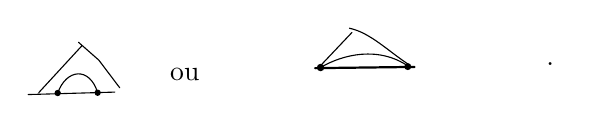
\begin{tikzpicture}[x=.78cm,y=.78cm,line cap=round,line join=round]
\draw (-.10,0)--(1.31,.04) (.07,.03)--(.77,.79) (.72,.85)--(1.05,.56)--(1.39,.11);
\draw (.38,.025) .. controls (.52,.42) and (.90,.46) .. (1.03,.03);
\fill (.38,.025) circle (.052) (1.03,.03) circle (.052);
\node at (2.45,.33) {ou};
\begin{scope}[shift={(4.66,.44)}]
\draw (-.03,0)--(.51,.57) (.47,.64) .. controls (.81,.57) and (1.12,.25) .. (1.45,.04);
\draw[line width=.8pt] (-.09,-.01)--(1.53,.01);
\draw (0,0) .. controls (.37,.22) and (.95,.35) .. (1.43,.02);
\fill (0,0) circle (.061) (1.42,.015) circle (.057);
\end{scope}
\node at (8.40,.49) {.};
\end{tikzpicture}}
ce qui me conduit à accepter des subdivisions de $\Delta^2$ en deux triangles comme ceci
\figure{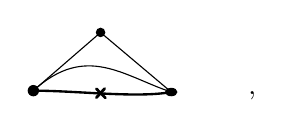
\begin{tikzpicture}[x=.88cm,y=.88cm,line cap=round,line join=round]
\draw (0,0)--(.97,.84)--(1.99,-.02);
\draw[line width=.85pt] (0,0) .. controls (.63,.00) and (1.50,-.11) .. (1.99,-.02);
\draw (0,0) .. controls (.76,.69) and (1.30,.21) .. (1.99,-.02);
\fill (0,0) circle (.082) (.97,.84) circle (.069) (1.99,-.02) ellipse (.09 and .061);
\draw[line width=1pt] (.91,.026)--(1.04,-.105) (.91,-.10)--(1.03,.031);
\node at (3.16,-.07) {,};
\end{tikzpicture}}
ce que personne ne \unsure{regardera} comme une subdivision simpliciale ! C'est le modèle des \uline{simplexes affines} dans un espace affine qui a guidé les gens, et il faut \unsure{utiliser}
\scanpage{13}\mspage{12}
ici la notion de raffinement \uline{stricte}. Dans \unsure{GP|GR} \uline{V} p. 19,20, il faut supposer, pour $F\overset{s}{\ll}\unsure{G|C}$, dans a) \deleted{que} [en plus de $\forall\,A\in F$, $G^A$ a un plus petit élément] que pour $A\in F$, $B\in G$, $A\cap B$ soit ou bien vide, ou une \deleted{\unsure{face de}} sous-strate de $A$ :
\deleted{En termes de la famille induite par $G$ sur $|F|$ (où on ne retient que les traces sur $|F|$ des $B\in G$ telles que $\mathring{B}\cap|F|\neq\unsure{\phi|\varnothing}$).} \deleted{cela signifie ceci} \deleted{si on veut que} \deleted{Cela signifie \unsure{aussi}}

Il faut faire \unsure{une|un} \unsure{pareille|pareil} \deleted{\unsure{strict}} \unsure{durcissement|changement|opération} pour la notion de compatibilité (la renforçant en ``compatibilité stricte'', ou ``polyédrale'') -- qui signifie que, \unsure{non seulement|bien seulement} $F\cup G$ est une \deleted{\unsure{famille}} \inserted{figure \unsure{ensembliste}}, admettant $F$ et $G$ comme sous-figure, mais que c'est une figure ensembliste \uline{polyédrale}.

En résumé, \deleted{pour} la formulation des axiomes spéciaux, il faut distinguer ceux relatifs aux ``ateliers polyédraux'', et ceux relatifs aux ``ateliers \unsure{spéciaux|spacieux}''.

Quand on en viendra \unsure{aux} plongements des $\mathrm{Fig}(\unsure{L|\mathcal{L}})$, dans le premier cas il faudra poser (pour les ateliers \unsure{polyédraux} ensemblistes, à ne pas confondre avec ateliers ensemblistes polyédraux, qui n'existent \unsure{plus} !)
% slanted
\margin{propriété qui \unsure{remplace|figure} \unsure{Axiome|Axiom} \unsure{des|du} \unsure{Cat PL|Cat P|Ch.} \unsure{VI|II} p.52}
que
\[
\deleted{\unsure{F}}\unsure{\mathrm{mulens}|\mathrm{mulont}|\mathrm{mulons}}(F)
\overset{\mathrm{pol}}{\ll}\mathrm{mulens}\,G\Longrightarrow F\ll G.
\]
\scanpage{14}\mspage{13}
\uline{Définition}\quad Un \unsure{ens|ens.} ordonné $I$ est dit \uline{polyédral} si deux éléments minorés ont un inf. \deleted{(NB si $I$ est fini, cel revient à ceci : l'ens \unsure{ordonné} $I_{\leq x}$ et $I$} \deleted{\inserted{(i.e. si}} \inserted{NB cela signifie que si}
$x,y\in I$ sont tels que $I_{\leq x}\cap I_{\leq y}\neq\unsure{\phi|\varnothing}$, alors $I_{\leq x}\cap I_{\leq y}$ a un plus grand élément. Quand \deleted{\illegible{3}}\inserted{\unsure{cet ens ord|cet ens est}} est inductif, (\unsure{par ex|p. ex.} \unsure{fini}) \deleted{est \unsure{filtrant}} il revient au \unsure{même|$\widetilde{\ }$} de dire que ledit \deleted{\unsure{ens}} $I_{\leq x}\cap I_{\leq y}$ est filtrant\inserted{\unsure{croiss.}}\unsure{,)} \deleted{\unsure{donc ceci ce}} signifie
\[
\begin{aligned}
&\forall\,x,y,x',y'\in I\text{ tels que }\ x',y'\leq x,y,\quad \exists\,z\in I\text{ tel que}\\
&\hspace{8em}x',y'\leq z\leq x,y
\end{aligned}
\]
% slanted
\margin{Cela signifie aussi, en termes \unsure{topolgiques|topologiques}, que l'intersection de deux parties fermées \uline{\unsure{strictmt|strict}} irréductibles est itou -- chose des plus remarquables \unsure{certes} !}

Sous cette forme, on voit que la condition est autoduale, et signifie donc aussi que deux \unsure{élément|éléments} majorés de $I$ ont un plus grand élément.

Donc \uline{Lemme} Supposons que $\forall\,x,\deleted{\unsure{y,x',y'}}x'\in I$ tels que $x'\leq x$, $I^{\mathrm{opp}}_{x'\leq\,\cdot\,\leq x}$ soit inductif. \deleted{Alors} (\unsure{p.ex.|p. ex.} fini). Alors si $I$ est polyédral, $I^{\mathrm{opp}}$ l'est, et l'inverse est vrai si les $I_{x'\leq\,\cdot\,\leq x}$ sont inductifs. \unsure{?}\unsure{à|--}.

Si \deleted{\unsure{Soit}} $\mathcal{A}=(\mathcal{F},\unsure{\leq^{\prime}|\leq},\ll)$ est un atelier, $F\in\unsure{\mathcal{J}|\mathcal{F}}$, la \uline{figure} \uline{\unsure{ou|$\sigma$}} $F$ est dite \uline{polyédrale} si $\widetilde{F}$ est \unsure{polyédral|polyédrale}, i.e. si deux strates de $F$ non disjointes ont comme intersection une strate de $F$. L'atelier $\mathcal A$ est dit \uline{polyédral} si \deleted{\unsure{tout}} figure de $\mathcal A$ est polyédral, i.e si on a ceci (en termes de $\unsure{M|\mathcal{M}}$) :

% slanted
\margin{(définition des ateliers polyédraux, ou condition de la stricte \unsure{intersection}}
\uline{At} \uline{pol} 1\quad $\forall\,X,Y\in M$, si $X\underset{M}{\mathrel{>\mkern-12mu<}}Y$ et $X$ et $Y$ non disjoints (i.e. $\{X,Y\}$ minoré dans $M$) alors \deleted{\unsure{on}} $\mathrm{Inf}^{M,\leq}(X,Y)$ existe.

Un ens. ordonné \inserted{$I$} est dit \uline{simplicial}, s'il est polyédral, et si pour tout $x\in I$, $S=I_{\leq x}$ est un \uline{simplexe combinatoire}, i.e. isomorphe à \deleted{\unsure{l'}}\inserted{un} ensemble ordonné ${\unsure{\mathcal{P}|\mathscr{P}}}^*(J)$ \inserted{($\mathcal P^*\unsure{[J]|(J)}={}$ ens. des parties \uline{non vides} de $J$)}, où $J$ est un ens \uline{fini}.

Pour un ens. ordonné $S$, il revient au $=$ de dire que $S$ est un simplexe combinatoire, ou que $S$ est \inserted{polyédral} fini, qu'il a un plus grand élément, et que chaque élément non minimal a au moins deux prédécesseurs. [Alors on voit par induction sur $\mathrm{card}\,S$ que \unsure{tt|tout} élément de $S$ est
\scanpage{15}\mspage{14}
le sup de\unsure{s} \inserted{l'ens des} éléments minimaux qu'il majore, et si $J$ est l'ens de ces éléments minimaux, on trouve $S\simeq{\unsure{\mathcal{P}|\mathscr P}}^{*}(J)$\unsure{...})
Une \uline{figure} \inserted{$F$} est dite (combinatoirement) \uline{simpliciale}, si $\widetilde F$ est \unsure{simpliciale|simplicial} -- i.e. si elle est polyédrale, et si ses strates sont des simplexes combinatoires. Un \uline{atelier} est dit \inserted{(combinatoirement)} \uline{simplicial} si \deleted{\unsure{toutes}} ses figures sont simpliciales, \unsure{i.e.} il satisfait, en plus de At pol 1 ci-dessus, la condition

\uline{At simp 1}\quad $\forall\,X\in\unsure{M|\mathcal M}$, \deleted{l'ens $\widetilde X=M_{\leq X}$ est un simplexe combinatoire, \illegible{1} dans $(M,\leq)$, alors $X$ a au moins deux prédécesseurs, i.e. $\partial X$ a au moins deux éléments maximaux} \deleted{\inserted{si $X$ n'est pas minimal}} $\partial X\overset{\mathrm{déf}}{=}\{Y\in M\mid Y<X\}$ est vide, \deleted{ou} \unsure{(i.e.} $X$ minimal dans $\deleted{\unsure{M}}(M,\leq)$) ou admet au moins deux éléments maximaux.

Je reviens aux axiomes complémentaires

% slanted
\margin{La formuler tout de suite sous forme de la \unsure{prop.} ?}
\uline{At C}\quad (\deleted{Axiome}\inserted{Critère} de \uline{compatibilité} des \uline{raffinements} \uline{des sous-figures}) Soient $X,Y,X',Y'$ \inserted{$\in M$}, avec $X'\ll X$, $Y'\ll Y$, $X\mathrel{>\mkern-12mu<}Y$. Soit $L=X\cap Y\left(=\widetilde X\cap\widetilde Y=\{Z\in M\mid Z\leq X,Y\}\right)$, Soient
$X'_L=X'\mathbin{.}L=\mathrm{Inf}^{\ll}(X,L)=\{X''\in\widetilde X'\mid X''\ll L\}$, et $Y'_L=Y'\mathbin{.}L=\ldots$, les raffinements de $L$ induits par $X',Y'$ respectivement. \deleted{Alors} [On sait déjà que $X'\mathrel{>\mkern-12mu<}Y'\Rightarrow X'_L\mathrel{>\mkern-12mu<}Y'_L$] Alors
\[
X'_L\mathrel{>\mkern-12mu<}Y'_L\Rightarrow X'\mathrel{>\mkern-12mu<}Y'.
\]

Cet axiome vise à la validité de la
\uline{Proposition}\quad Soient $F,\unsure{G|C},F',G'\in\mathcal{F}$, avec $F'\ll F$, $G'\ll G$, $F\mathrel{>\mkern-12mu<}G$ \unsure{(i.e.|(lire} $F,\unsure{G|L}$ sous-figures d'une $=$ figure $H$). Soit $L=F\cap G$, $F'_L=F'\deleted{\unsure{{}_L|\cap}}\mathbin{.}L$, $G'=G'\deleted{{}_L}\mathbin{.}L$. Alors
\[
F'\mathrel{>\mkern-12mu<}G'\Longleftrightarrow F'_L\mathrel{>\mkern-12mu<}G'_L.
\]
\scanpage{16}\mspage{15}
Au point de vue ensembliste, pour les supports des \unsure{Mulons|Mulens|Mulont} correspondants, on trouve la figure \unsure{suivante} (où $H=F\cup\unsure{G|C}$)
\diagram{\begin{tikzcd}[ampersand replacement=\&,row sep=1.6em,column sep=.75em]
\& \& \mathrm{Omb}\,H \arrow[dl,dash]\arrow[dr,dash] \& \& \\
\& \mathrm{Omb}\,F \arrow[dl,dash]\arrow[dr,dash] \& \& \mathrm{Omb}\,G \arrow[dl,dash]\arrow[dr,dash] \& \\
|[yshift=-.30em]|\mathrm{Omb}\,F' \arrow[dr,dash] \& \& \mathrm{Omb}\,L \arrow[dl,dash]\arrow[dr,dash] \& \& |[yshift=-.30em]|\mathrm{Omb}\,G' \arrow[dl,dash] \\
\& \mathrm{Omb}\,F'_L \& \& \mathrm{Omb}\,G'_L \&
\end{tikzcd}}

Où ch. \deleted{\unsure{que|quel}} des trois carrés est cartésien. \unsure{Itou|Item} pour les \unsure{déployements|déployement|déploiements}
\diagram{\begin{tikzcd}[ampersand replacement=\&,row sep=1.05em,column sep=.8em]
\& \& \widetilde H \& \& \\
\& \widetilde F \arrow[ur,hook] \& \& \widetilde G \arrow[ul,hook'] \& \\
|[yshift=-1.45em]|\widetilde F' \arrow[ur] \& \& \widetilde L\arrow[ul,hook']\arrow[ur,hook] \& \& |[yshift=-.45em]|\widetilde G' \arrow[ul] \\
\& |[yshift=-.65em]|\widetilde F'_L \arrow[ul,hook']\arrow[ur] \& \& \widetilde G'_L \arrow[ul]\arrow[ur,hook] \&
\end{tikzcd}}

La compatibilité de \deleted{$\unsure{F}$} $F'$ et $G'$ signifie que $\forall\,x'\in\widetilde F',\deleted{\unsure{a}}y'\in\widetilde G'$, on a $x'\mathrel{>\mkern-12mu<}y$ -- et la proposition dit qu'il suffit de le vérifier pour les strates $x',y'$ tels que $x'\in\widetilde F'_L$, $y'\in\widetilde G'_L$, i.e. telles que $\deleted{\unsure{F'}}x'\ll\deleted{\unsure{G}}L,\deleted{\unsure{y'\ll G}}\inserted{y''\ll L}$ (ce qui \unsure{équivaut} d'ailleurs à \deleted{$x'\ll G$}$x'\ll G$, $y'\ll F$). \deleted{\unsure{R}} \unsure{Signalons} la \unsure{conséquence|consigne}

\noindent\begin{tabular}{|p{.93\linewidth}}
\uline{At} D\quad (\deleted{Axiome}\inserted{Critère} de \uline{disjonction des raffinements} \uline{des sous-figures}) Soient $x,y,x',y'\in\unsure{M|\mathcal M}$, avec $x'\ll x\unsure{{}^{4}|{}^{a}|{}^{+}}$, $y'\ll y$, $x\mathrel{>\mkern-12mu<}y$. Soit $L=x\cap y$. [On sait déjà que $x'\parallel y'\Rightarrow x'_L\parallel y'_L$] Alors
\[
x'_L\parallel y'_L\Rightarrow x'\parallel y'
\]
\end{tabular}
\scanpage{17}\mspage{16}
\unsure{Vise|Visa} \unsure{à|:} la validité de la
\uline{Proposition}\quad \unsure{Données} comme \unsure{dans|ds} prop. précédente. Alors
\[
F'\parallel{\unsure{G|C}}'\Longleftrightarrow F'_L\parallel G'_L
\]
% slanted
\margin{cf aussi Cor. \unsure{2|5} (\unsure{lemme} ? V. \unsure{21|2.1})}
\uline{Corollaire} 1 \inserted{(At $D_0$)} Soient $F,G,F',G'$ avec $F\parallel G$, $F'\ll F$, $G'\ll G$, alors $F'\parallel G'$.

\uline{At} \uline{pol} \unsure{1|2} (\deleted{Axiome}\inserted{Critère} de \uline{compatibilité pour ateliers} \uline{polyédraux}) Soient $X,Y\in\unsure{M|\mathcal M}$. On ne suppose pas $X,Y$ compatibles, on introduit pourtant $L\deleted{\unsure{=}}\inserted{=X\cap Y=}\mathop{\mathrm{Sup}}\limits_{Z\in\widetilde X\cap\widetilde Y}Z$, \deleted{tel} \inserted{figure telle} que $\widetilde{\deleted{\unsure{I}}L}=\widetilde X\cap\widetilde Y$. Supposons que pour tout $X',Y'\in\deleted{\unsure{\mathcal M}}M$, avec
$X'\ll X$, $Y'\ll Y$, $\deleted{\unsure{X'\parallel L,\ Y'\parallel L}}X'_L=0$, $Y'_L=0$ on ait
\[
X'\parallel Y'.
\]
% slanted
\margin{On en voit il \unsure{me semble}, des \unsure{tas} \unsure{d'}axiomes \unsure{supplém.}, qui \illegible{1} une \unsure{cond.} \uline{néc.} \uline{et suff.} de la compatibilité -- \deleted{\illegible{1}} \deleted{\unsure{indiquer} aussi l'axiome At $D_0$}}
\deleted{Alors} Supposons de plus que $\deleted{\unsure{X'_L,\ Y'_L}}\inserted{L=\unsure{\phi|\varnothing}\text{ ou }}L\in M$ i.e. $\{X,Y\}$ \inserted{\deleted{\unsure{est}} \unsure{n'est} pas minoré \uline{ou}} admet\deleted{tent} un $\mathrm{Inf}$ dans $(M,\leq)$. Alors $X\mathrel{>\mkern-12mu<}Y$.

Vise à la validité de la proposition
\uline{Prop.} (Moyennant \uline{At} \uline{pol}) Soient $F,G\in\unsure{\mathcal F|\mathscr F}$. On ne suppose pas $F\mathrel{>\mkern-12mu<}G$, soit $L=F.G$. \deleted{\unsure{Supp}} Alors $F\mathrel{>\mkern-12mu<}G$ \unsure{ssi} les conditions suivantes sont satisfaites :

(i) $\forall\,x\in\widetilde F$, $y\in\widetilde G$, \deleted{\unsure{avec}} tels que $\{\deleted{\unsure{x'}}x,y\}$ soit minoré dans $M$, $x\cap y\in M$, i.e. $\deleted{\unsure{\mathrm{Inf}\,\mathrm{de}_{\leq}|\mathrm{Inf}^{\ll}|\mathrm{Inf}^{\leq}}}\widetilde x\cap\widetilde y$ est vide ou a un plus grand élément

(ii) $\forall\,\deleted{\unsure{x,y|x\parallel}}x,y\in M$, $\deleted{\unsure{\mathrel{>\mkern-12mu<}|x}}$ avec $x\ll F$, $y\ll G$, $\deleted{\unsure{x\parallel L}}x_L=\phi$, $y_L=\phi$, on \deleted{ait} a $x\parallel y$
